\chapter{Технические решения}
\label{chap:tech}
Для реализации всех алгоритмов классификации и кластеризации используется открытая библиотека Weka\footnote{http://www.cs.waikato.ac.nz/ml/weka/}. Основным языком реализации была выбрана Java\footnote{http://java.com} в силу своей распространенности и мультиплатформенности. Для работы с ``Википедией'' применяется библиотека wikixmlj\footnote{http://code.google.com/p/wikixmlj/}. Для работы с ``Твиттером'' применяется библиотека twitter4j\footnote{http://twitter4j.org/en/index.html}.

Итоговое решение можно разделить на следующие части: часть для работы с ``Твиттеров'', часть для работы с ``Википедией'', часть содержащая алгоритм классификации и тестирования. Для реализации контекстного классификатора был создан класс ContextClassifier, реализующий класс Classifier библиотеки Weka. В качестве параметров данного классификатора выступают фабрика\footnote{http://ru.wikipedia.org/wiki/Абстрактная\_фабрика\_(шаблон_проектирования)} для создания базовых классификаторов, фабрика алгоритмов кластеризации, модель выделения признаков из текста. Модель выделения признаков из текста реализована в виде наследника класса Filter библиотеки Weka.   

Диаграмму классов алгоритмов классификации можно увидеть на Рис. \ref{fig:uml-classifiers}, кластеризации на Рис. \ref{fig:uml-clusterers}, выделения признаков из текста на Рис. \ref{fig:uml-models}.

% http://yuml.me/diagram/plain/class/[Classifier|buildClassifier(data);classifyInstance(instance)]^-[ContextClassifier|classifier;clusterer;wordModel],[Classifier|buildClassifier(data);classifyInstance(instance)]^-[NaiveBayes],[Classifier|buildClassifier(data);classifyInstance(instance)]^-[MISVM],[Classifier|buildClassifier(data);classifyInstance(instance)]^-[J48]

\begin{figure}[h!]
  \centering
    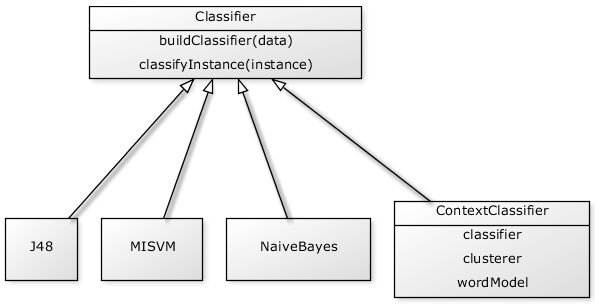
\includegraphics[width=0.7\textwidth]{uml/classifiers}
    \caption{Классы для классификации}
    \label{fig:uml-classifiers}
\end{figure}

% http://yuml.me/diagram/plain/class/[Filter]^-[MapFilter|map(data)],[MapFilter|map(data)]^-[WikiTextModel],[Filter]^-[StringToWordVector]

\begin{figure}[h!]
  \centering
    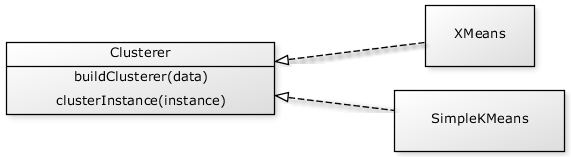
\includegraphics[width=0.7\textwidth]{uml/clusterers}
    \caption{Классы для кластеризации}
    \label{fig:uml-clusterers}
\end{figure}

% http://yuml.me/diagram/plain/class/[Clusterer|buildClusterer(data);clusterInstance(instance)]^-.-[SimpleKMeans],[Clusterer|buildClusterer(data);clusterInstance(instance)]^-.-[XMeans]

\begin{figure}[h!]
  \centering
    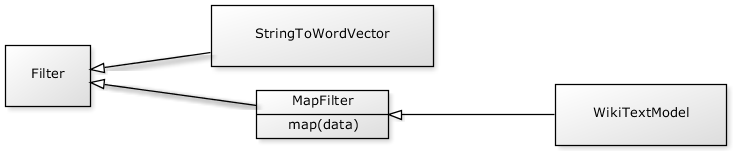
\includegraphics[width=0.7\textwidth]{uml/models}
    \caption{Классы для выделения признаков из текста}
    \label{fig:uml-models}
\end{figure}
